\documentclass{standalone}

\usepackage{tikz}
\usepackage{standalone}
\usetikzlibrary{calc}

\begin{document}

    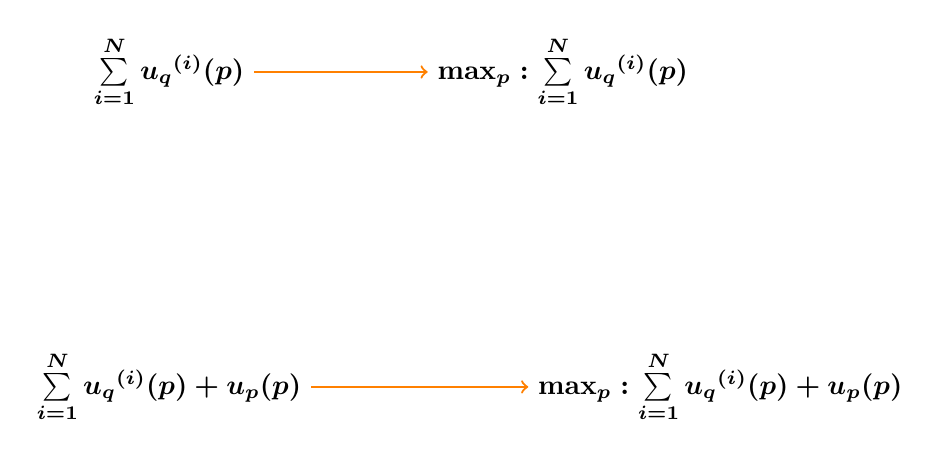
\begin{tikzpicture}

    \tikzstyle{state}=[minimum width=1cm, font=\boldmath];
    

	\node (u) at (0, 0) [state] {$\sum\limits_{i=1} ^ {N} {u_q}^{(i)} (p)$};
	\pause
    \node (max) at (5, 0) [state] {$\max_p: \sum\limits_{i=1} ^ {N} {u_q}^{(i)} (p)$};
    \draw (u) edge[out=0, in=180, ->, thick, orange] node [above] {} (max);

    \pause
    \node (u_e) at (0, -4) [state] {$\sum\limits_{i=1} ^ {N} {u_q}^{(i)} (p) + u_p(p)$};

    \node (max_e) at (7, -4) [state] {$\max_p: \sum\limits_{i=1} ^ {N} {u_q}^{(i)} (p) + u_p(p)$};
    \draw (u_e) edge[out=0, in=180, ->, thick, orange] node [above] {} (max_e);
    
    \end{tikzpicture}

\end{document}